\documentclass{article}
\usepackage[utf8]{inputenc}
\usepackage[T1]{fontenc}
\usepackage[english]{babel}
\usepackage{fancyhdr}
\usepackage{svg}
\usepackage{hyperref}
\usepackage{graphicx}
\usepackage{array}
\usepackage{tabularx}

\title{
        \vspace{-2cm}
        \begin{center}
                
\includegraphics[width=0.4\textwidth]{asset/logo.png} % ← change le nom et la taille selon ton image
        \end{center}
        \vspace{1cm}
        \textbf{Hypermedia Applicaton \\ Design Report}
}
\author{Yuto Yamaguchi \href{mailto:yuto.yamaguchi@mail.polimi.it}{yuto.yamaguchi@mail.polimi.it} \\
Xavier Anicito \href{mailto:xavierandre.anicito@mail.polimi.it}{xavierandre.anicito@mail.polimi.it} \\
Ewan Decima \href{mailto:ewangabriel.decima@mail.polimi.it}{ewangabriel.decima@mail.polimi.it}
}
\date{April 2025}








% Footer configuration
\pagestyle{fancy}
\fancyhf{} % clear all header and footer fields
\fancyfoot[R]{Yuto Yamagachi, Xavier Anicito, Ewan Decima}
\renewcommand{\headrulewidth}{0pt}
\renewcommand{\footrulewidth}{0.4pt}

\begin{document}

\maketitle
\tableofcontents
\newpage

\section{Abstract}

The purpose of this design report is to provide a comprehensive overview of the key elements and decisions made
during the website implementation for a yoga center. The report meticulously outlines the primary design choices
made throughout the project, supported by relevant models, schemas, and use case scenarios. Furthermore,
it presents the conceptual and logical structure of the database, which underpins user interaction,
class scheduling, subscription management, and content delivery functionalities.

\newpage

\section{Conceptual design}
This section presents an exhaustive summary of the conceptual design principles applied to the website.
It meticulously examines the decision-making process governing the content selection, its structuring into pages,
and the seamless navigation between them. The subsequent sections delve into the intricacies of these decisions,
providing a comprehensive explanation and analysis.

\subsection{C-IDM Diagram}
In this subsection, the Content Interaction Dialogue Model (C-IDM) is introduced as a model that represents the website
as a conversation between the user and the application. This model elucidates the nature of the dialogue,
including its classification, inter-relationships, and grouping of conversation topics. Additionally,
it provides insights into the content that can be discussed within each category.

\begin{figure}[h]
        \centering
        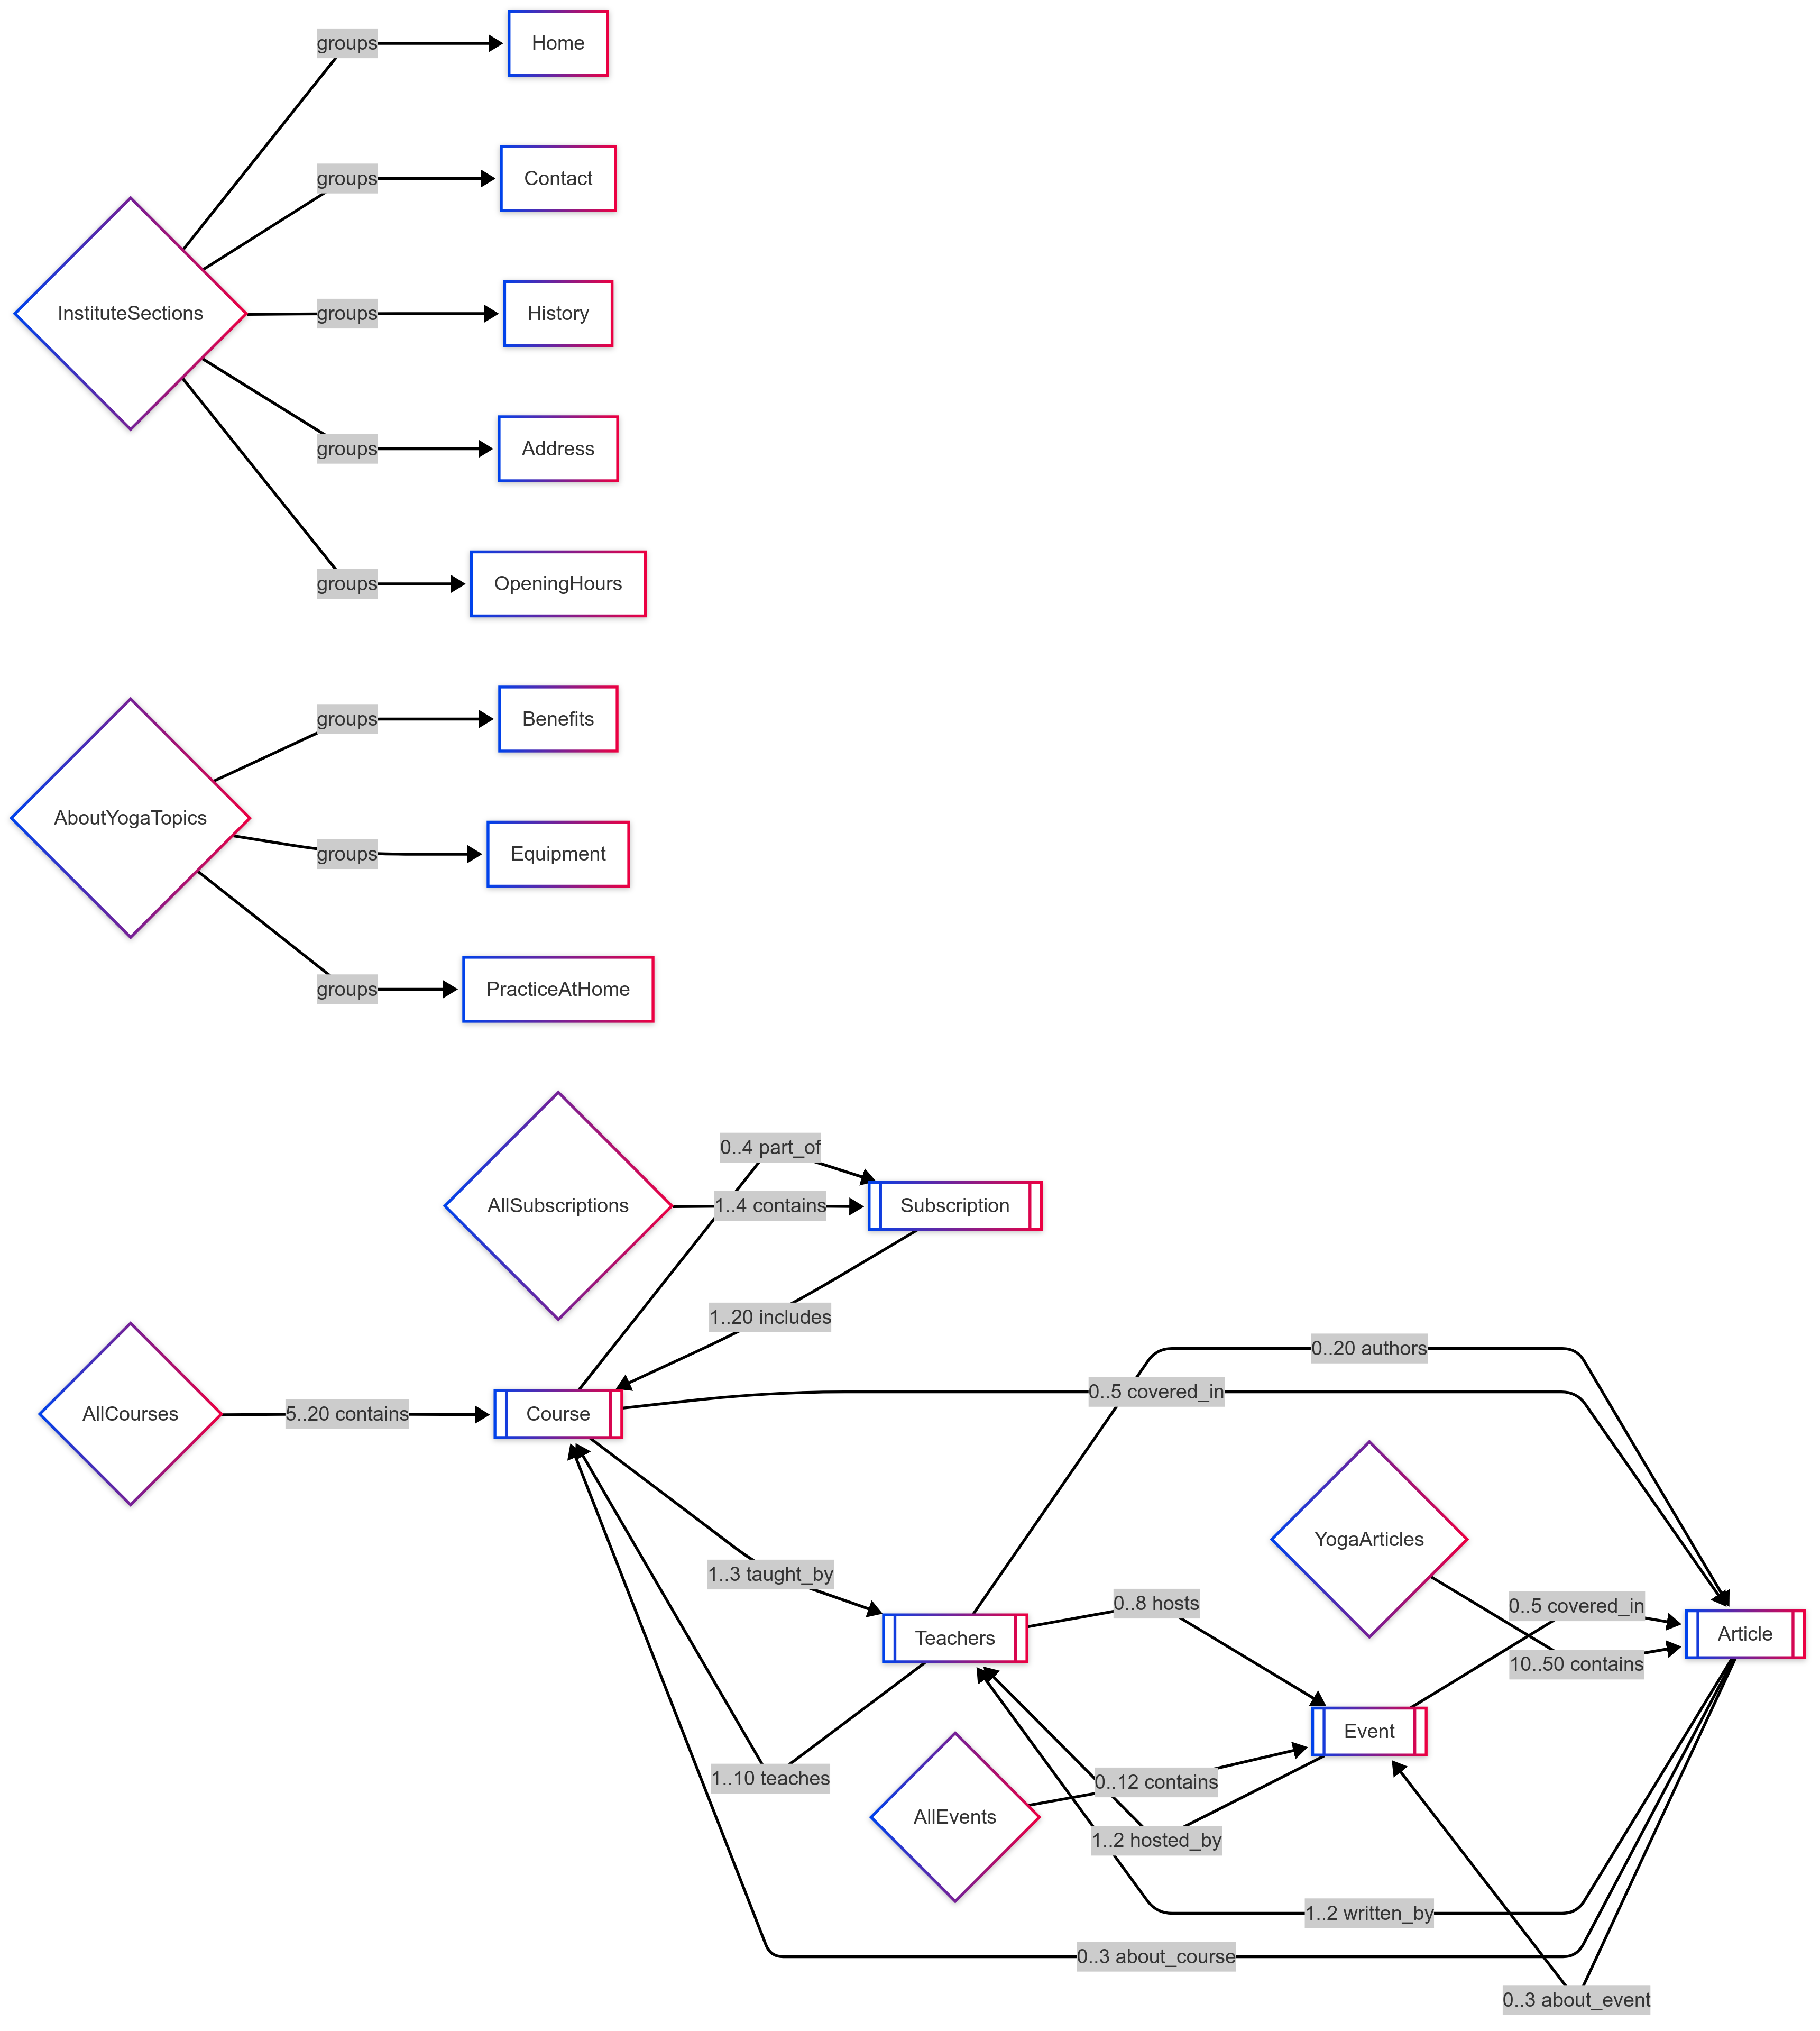
\includegraphics[width=0.8\textwidth]{asset/c_idm_scheme}
        \caption{C-IDM Diagram}
\end{figure}

\subsection{Content-in-the small Tables}

\subsubsection{Topics}


\begin{center}
        \begin{tabularx}{\textwidth}{|>{\bfseries}l|X|}
                \hline
                Topic: & \textbf{Home} \\
                \hline
                Title: & text  (max 50 chars)\\
                \hline
                NewCustomerOffer: & text \\
                \hline
                FeaturedPanel: & text \\
                \hline
                DiscoverCourseLink: & URL \\
                \hline
                ContactLink: & URL \\
                \hline

        \end{tabularx}
        \caption{Table: Home}
\end{center}

\begin{center}
        \begin{tabularx}{\textwidth}{|>{\bfseries}l|X|}
                \hline
                Topic: & \textbf{Contact} \\
                \hline
                ContactInfo: & text  (max 200 chars)\\
                \hline
                ContactFormFiels: & List of text \\
                \hline
                SocialMediaLinks: & List of text \\
                \hline

        \end{tabularx}
        \caption{Table: Contact}
\end{center}


\begin{center}
        \begin{tabularx}{\textwidth}{|>{\bfseries}l|X|}
                \hline
                Topic: & \textbf{Histroy} \\
                \hline
                Title: & text  (max 200 chars)\\
                \hline
                Content: & text (max 1000 chars)\\
                \hline
                FounderImages: & List of {Image} \\
                \hline

        \end{tabularx}
        \caption{Table: History}
\end{center}


\begin{center}
        \begin{tabularx}{\textwidth}{|>{\bfseries}l|X|}
                \hline
                Topic: & \textbf{Address} \\
                \hline
                AddressText: & text  (max 200 chars)\\
                \hline
                MapEmbed: & interactive map \\
                \hline
                PublicTransportInfo: & text (max 500 chars)\\
                \hline
                OpenHoursLink: & URL \\
                \hline

        \end{tabularx}
        \caption{Table: History}
\end{center}

\begin{center}
        \begin{tabularx}{\textwidth}{|>{\bfseries}l|X|}
                \hline
                Topic: & \textbf{PracticeAtHome} \\
                \hline
                Title: & text  (max 200 chars)\\
                \hline
                Content: & text (max 500 chars) \\
                \hline
                Exercice: & text (max 500 chars)\\
                \hline
                OpenHoursLink: & URL \\
                \hline
                VideoLinks: & List of URLs \\
                \hline
                SafetyGuidelines: & text (max 500 chars) \\
                \hline


        \end{tabularx}
        \caption{Table: Practice at home}
\end{center}

\begin{center}
        \begin{tabularx}{\textwidth}{|>{\bfseries}l|X|}
                \hline
                Topic: & \textbf{OpeningHours} \\
                \hline
                WeeklySchedule: & List of {(Day, CourseName, Time)}  (max 200 chars)\\
                \hline
                PrivateCourseBookingLink: & URL \\
                \hline


        \end{tabularx}
        \caption{Table: Opening Hours}
\end{center}

\begin{center}
        \begin{tabularx}{\textwidth}{|>{\bfseries}l|X|}
                \hline
                Topic: & \textbf{Benefit} \\
                \hline
                Title: & text  (max 200 chars)\\
                \hline
                Content: & text (max 500 chars) \\
                \hline
                FeatureList: & List of {(Benefit, Description)} (max 500 chars)\\
                \hline
                RelatedLink: & URL \\
                \hline

        \end{tabularx}
        \caption{Table: Benefit}
\end{center}


\begin{center}
        \begin{tabularx}{\textwidth}{|>{\bfseries}l|X|}
                \hline
                Topic: & \textbf{Equipement} \\
                \hline
                Title: & text  (max 200 chars)\\
                \hline
                Content: & text (max 500 chars) \\
                \hline
                FeatureList: & List of {(Benefit, Description)} (max 500 chars)\\
                \hline
                RelatedLink: & URL \\
                \hline

        \end{tabularx}
        \caption{Table: Equipement}
\end{center}

\subsubsection{Kind of Topic}

\begin{center}
        \begin{tabularx}{\textwidth}{|>{\bfseries}l|X|}
                \hline
                Kind of topic: & \textbf{Course} \\
                \hline
                Title: & text  (max 200 chars)\\
                \hline
                Image: & image \\
                \hline
                Description: & text (max 500 chars) \\
                \hline
                Goal: & text (max 200 chars) \\
                \hline
                Timetable: & List of {(Day, Time)}\\
                \hline
                Price: & currency \\
                \hline
                IntroVideoUrl: & URL \\
                \hline
                TaughtBy: & List of {Teachers, Link} \\
                \hline
                PartOfSubscription: & List of {(Subscription, Link)} \\
                \hline
                CoveredInArticle: & List of {(Article, Link)}\\
                \hline
        \end{tabularx}
        \caption{Table: Course}
\end{center}

\begin{center}
        \begin{tabularx}{\textwidth}{|>{\bfseries}l|X|}
                \hline
                Kind of Topic: & \textbf{Subscription} \\
                \hline
                Name: & text  (max 200 chars)\\
                \hline
                Type: & text (max 200 chars) \\
                \hline
                TotalCourse: & integer \\
                \hline
                Price: & Currency \\
                \hline
                Link: & URL \\
                \hline
                ContactLink: & URL \\
                \hline
                Details: & text (max 500 chars) \\
                \hline
                CoursesIncluded: & List of {(CourseTitle, Link)}\\
                \hline
        \end{tabularx}
        \caption{Table: Equipement}
\end{center}

\begin{center}
        \begin{tabularx}{\textwidth}{|>{\bfseries}l|X|}
                \hline
                Kind of Topic: & \textbf{Event} \\
                \hline
                Title: & text  (max 200 chars)\\
                \hline
                Image: & Image \\
                \hline
                Date: Timestamp \\
                \hline
                Description: & text (max 500 chars) \\
                \hline
                Location: & text (max 500 chars) \\
                \hline
                BookingLink: & URL \\
                \hline
                HostedBy: & List of {(Teachers, Link)} \\
                \hline
                CoveredInArticles: List of {(Article, Link)}\\
                \hline

        \end{tabularx}
        \caption{Table: Event}
\end{center}

\begin{center}
        \begin{tabularx}{\textwidth}{|>{\bfseries}l|X|}
                \hline
                Kind of Topic: & \textbf{Teacher} \\
                \hline
                Name: & text  (max 200 chars)\\
                \hline
                Photo: & Image \\
                \hline
                Biography: & text (max 500 chars) \\
                \hline
                Certificates: & List of {Image or Text} \\
                \hline
                CoursesTaught: & List of {(Course, Link)} \\
                \hline
                SocialMedias: & List of {URL} \\
                \hline
                HostedEvents: & List of {(Event, Link)}
                \hline
                AuthoredArticles: & List of {(Article, Link)} \\
                \hline

        \end{tabularx}
        \caption{Table: Teacher}
\end{center}
\begin{center}
        \begin{tabularx}{\textwidth}{|>{\bfseries}l|X|}
                \hline
                Kind of Topic: & \textbf{Article} \\
                \hline
                Title: & text  (max 200 chars)\\
                \hline
                ThumbnailImage: & Image \\
                \hline
                Snippet: & text (max 200 chars) \\
                \hline
                FullText: & text \\
                \hline
                Authors: & List of {Text or (Teachers, Link)}
                \hline
                PublishDate: & Date (Timestamp) \\
                \hline
                AboutCourses: & List of {Course, Link} \\
                \hline
                AboutEvents: & List of {(Event, Link)}
                \hline
        \end{tabularx}
        \caption{Table: Article}
\end{center}

\subsubsection{Group of Topics}
\begin{center}
        \begin{tabularx}{\textwidth}{|>{\bfseries}l|X|}
                \hline
                Group: & \textbf{AllCourses} \\
                \hline
                Title: & text  (max 200 chars)\\
                \hline
                Description: & text (max 500 chars) \\
                \hline
                MembersPreview: & List of {(Course, Thumbnail, Title, Price)} \\
                \hline

        \end{tabularx}
        \caption{Table: All Courses }
\end{center}

\begin{center}
        \begin{tabularx}{\textwidth}{|>{\bfseries}l|X|}
                \hline
                Group: & \textbf{AllSubscription} \\
                \hline
                Title: & text  (max 200 chars)\\
                \hline
                Description: & text (max 500 chars) \\
                \hline
                MembersPreview: & List of {(Subscription, Name, TotalCourses, Price)} \\
                \hline

        \end{tabularx}
        \caption{Table: All Subscriptions }
\end{center}

\begin{center}
        \begin{tabularx}{\textwidth}{|>{\bfseries}l|X|}
                \hline
                Group: & \textbf{AllEvents} \\
                \hline
                Title: & text  (max 200 chars)\\
                \hline
                Description: & text (max 500 chars) \\
                \hline
                MembersPreview: & List of {(Event, Thumbnail, Title, Date)} \\
                \hline

        \end{tabularx}
        \caption{Table: All Events }
\end{center}

\begin{center}
        \begin{tabularx}{\textwidth}{|>{\bfseries}l|X|}
                \hline
                Group: & \textbf{AllTeachers} \\
                \hline
                Title: & text  (max 200 chars)\\
                \hline
                Description: & text (max 500 chars) \\
                \hline
                MembersPreview: & List of {(Teacher, Names, CoursesTaught)} \\
                \hline

        \end{tabularx}
        \caption{Table: All Teachers }
\end{center}

\begin{center}
        \begin{tabularx}{\textwidth}{|>{\bfseries}l|X|}
                \hline
                Group: & \textbf{InstitueSection} \\
                \hline
                Title: & text  (max 200 chars)\\
                \hline
                Description: & text (max 500 chars) \\
                \hline
                MembersPreview: & List of {(SectionTitle, Snippet)} \\
                \hline

        \end{tabularx}
\end{center}


\begin{center}
        \begin{tabularx}{\textwidth}{|>{\bfseries}l|X|}
                \hline
                Group: & \textbf{AboutYogaTopics} \\
                \hline
                Title: & text  (max 200 chars)\\
                \hline
                Description: & text (max 500 chars) \\
                \hline
                MembersPreview: & List of {(TopicTitle, Link)} \\
                \hline

        \end{tabularx}
        \caption{Table: About Yoga Topics }
\end{center}

\begin{center}
        \begin{tabularx}{\textwidth}{|>{\bfseries}l|X|}
                \hline
                Group: & \textbf{AllYogaArticles} \\
                \hline
                Title: & text  (max 200 chars)\\
                \hline
                Description: & text (max 500 chars) \\
                \hline
                MembersPreview: & List of {(Article, Thumbnail, Title, PublishDate)} \\
                \hline

        \end{tabularx}
        \caption{Table: All Yoga Articles}
\end{center}



\section{Final Commented Screenshots}

\section{Interaction Scenarios}

\section{Database Design}

This section presents the design of the database for the website to be implemented. Indeed, it manages students, teachers, courses, subscriptions, feedback,
equipment, events, and articles. The schema includes detailed relationships between entities, such as students
enrolling in courses, courses requiring specific equipment, and subscriptions granting access to various learning materials. JSON fields are used for flexible
data such as certificates, goals, and social media links.

\subsection{Explanation of Relationship Symbols}

The following notation is used in the Entity-Relationship (ER) diagrams, following the Mermaid syntax conventions that
you can check on : \href{https://mermaid.js.org/syntax/entityRelationshipDiagram.html}{mermaid.js.org}

\subsection{Entity-Relation Diagram}

\begin{figure}[h]
        \centering
        \includesvg[width=0.8\textwidth]{asset/database_e_r_diagram.png}
        \caption{E-R Diagram}
\end{figure}





\end{document}
